\documentclass[10pt,xcolor=dvipsnames]{beamer}

\usetheme{Warsaw}
\usepackage{amsmath}
\usepackage{bm}
\usepackage{tikz}
\usepackage{graphicx}
\usepackage{booktabs}
\usepackage{acronym}
\usepackage{ifthen} 
\usepackage{xcolor} 

\usetikzlibrary{calc}
\usetikzlibrary{fit}
\usetikzlibrary{arrows.meta}
\usetikzlibrary{scopes}
\usetikzlibrary{positioning}


\acrodef{DNS}{Domain Name System}
\acrodef{DN}{Domain Name}
\acrodef{DGAMLM}{DGA Machine Learning Model}
\acrodef{DGAIDS}{DGA-based Intrusion Detection System}

\acrodef{TLD}{Top Level Domain}
\acrodef{ICANN}{Internet Corporation for Assigned Names and Numbers}

\acrodef{TN}{True Negative}
\acrodef{FP}{False Positive}
\acrodef{FPCD}{False Positive Classified Domain}
\acrodef{FPh}[FPs/h]{False Positives per hour}
\acrodef{FN}{False Negative}
\acrodef{TP}{True Positive}
\acrodef{NXD}[NX domain]{Not-Existent Domain}
\acrodef{EXD}{Existent Domain}

\acrodef{TPR}{True Positive Ratio}
\acrodef{FPR}{False Positive Ratio}

\acrodef{DNSp}[DNS packet]{DNS packet}

\acrodef{PP}[P\textit{P}]{Predicted Positives}
\acrodef{AP}[A\textit{P}]{Actual Positives}
\acrodef{PN}[P\textit{N}]{Predicted Negatives}
\acrodef{AN}[A\textit{N}]{Actual Negatives}

\acrodef{NA}{True No-alarm}
\acrodef{FA}{False Alarm}
\acrodef{MA}{Missed Alarm}
\acrodef{TA}{True Alarm}

\acrodef{NCD}[nCD]{Negatively Classified Domain}
\acrodef{PCD}[pCD]{Positively Classified Domain}

\acrodef{NX}[NX]{Not-eXistent}
\acrodef{DGA}{Domain Ge\-neration Algorithm}
\acrodef{AGD}{Algorithmically-Generated Domain}
\acrodef{uNXd}[uNXd]{unique NX domain}
\acrodef{uNXp}[uNXd]{unique NX packet}
\acrodef{mAG}{malicious Algorithmically-Generated}
\acrodef{mAGD}{malicious Algorithmically-Generated Domain}
\acrodef{mAGDc}[mAGD classifier]{mAGD classifier}
\acrodef{mAGDnn}{malicious Algorithmically-Generated Domain neural network}
\acrodef{mAGD-NIDS}{\ac{mAGD}-\ac{NIDS}}

\acrodef{IDS}{Intrusion Detection System}
\acrodef{NID}{Network Intrusion Detection}
\acrodef{CC}[C\&C]{Command and Control}
\acrodef{NDS}{Network Data Set}
\acrodef{MCFP}{Malware Capture Facility Project}
\acrodef{PCAP}{Packet Capture}
\acrodef{ML}{Machine Learning}
\acrodef{ML-IDS}{Machine Learning Intrusion Detection System}
\acrodef{TLD}{Top Level Domain}
\acrodef{eTLD}{effective Top Level Domain}
\acrodef{IP}{Internet protocol}

\acrodef{LSTM}{Long Short-Term Memory}
\acrodef{RNN}{Recurrent Neural Network}
\acrodef{CNN}{Convolutional Neural Network}
\acrodef{GAN}{Generative Adversarial Networks}

\acrodef{IANA}{Internet Assigned Numbers Authority}
\acrodef{ICANN}{Internet Corporation for Assigned Names and Numbers}

\acrodef{LLR}{Log-Likelihood Ratio}
\acrodef{hD}{healthy Domain}
\acrodef{nD}{normal Domain}
\acrodef{SVM}{Support Vector Machine}
\acrodef{RF}{Random Forest}
\acrodef{SOC}{security Operations Center}
\acrodef{NIDS}{Network Intrusion Detection System}
\acrodef{DNS-NIDS}{Domain Name System Network-IDS}
\acrodef{DGA-NIDS}{DGA Network-IDS}
\acrodef{hC}[hC]{healthy capture}
\acrodef{iC}[IC]{\textit{infected} capture}
\acrodef{nIC}[nIC]{non-DGA infected capture}
\acrodef{dgaIC}[dgaIC]{DGA infected capture}
\acrodef{VM}[VM]{Virtual Machine}
\acrodef{dNN}[dNN]{DGA Neural Network}
\acrodef{URL}[URL]{Uniform Resource Locator}

\tikzset{
  comp/.style = {
    minimum width  = 8cm,
    minimum height = 4.5cm,
    text width     = 8cm,
    inner sep      = 0pt,
    text           = black,
    align          = center,
    font           = \Huge,
    transform shape,
    thick
  },
  monitor/.style = {draw = none},%, xscale = 18/16, yscale = 11/9},
  display/.style = {fill=white},%shading = axis},%, left color = black!60, right color = black},
  ut/.style      = {fill = gray}
}



\definecolor{colordns}{RGB}{150, 150, 150}
\definecolor{colordns_green}{RGB}{150, 150, 150}
\definecolor{colordns_red}{RGB}{150, 150, 150}

\tikzset{
  dnsq/.pic={
      % \draw[fill=black!10] (0.25,0) -- (2.0,0) -- (2.5,0.5) -- (2.0,1) -- (0.25,1) -- (0.25,0);
      \node[draw, inner sep=2.5mm, rounded corners,minimum width=2.5cm, minimum height=1cm,anchor=center,align=center] at (0,0) (-node) {\tikzpictext};
      % \node[fill=white, inner sep=1pt] at (1.25,1) {DNS};
  },
  dnsr/.pic={
      % \draw[fill=black!10] (0,0.5) -- (0.5,0) -- (2.25,0) -- (2.25,1.0) -- (0.5,1.0) -- (0,0.5);
      \node[draw,rounded corners,minimum width=2.5cm, minimum height=1.25cm] (-node) {\tikzpictext};
      \node[fill=white, inner sep=1pt] at (1.25,1) {DNS};
      % \node[anchor=north, inner sep=2pt] at (1.25,0) {response};
  },
  ggrid/.pic={
    \draw[step=1cm, gray!50, very thin] (0,0) grid (16,9);

    \foreach \x in {1, ..., 15}
      \draw[gray, very thin] (\x, 0) -- (\x, 0) node[anchor=south,font=\small,inner sep=0] {\x};
    
    \foreach \y in {1,...,8} {
      \draw[gray, very thin] (0, \y) -- (0, \y) node[anchor=west,font=\small,inner sep=0] {\y};
      }
      \draw[black!50] (8, 0) -- (8, 9);
      \draw[black!50] (0, 4.5) -- (16, 4.5);
  },
  nnpic/.pic={
    \node[draw, rounded corners, text width=1.5cm, inner sep=0.2cm, font=\Huge] (svm) {
\includegraphics[width=\textwidth]{ml.pdf}};
  },
  seagull/.pic={
    \coordinate (-origin) at (0,0);

    \foreach[count=\i] \angle in {1,2,3,4,5,6} {
      \node[text width=1cm,inner sep=0] (-t\i) at (60*\angle:2cm) {\resizebox{\textwidth}{!}{
\includegraphics[]{laptop-svgrepo-com_no.pdf}}};
      \node at (60*\angle:2cm) {\i};
    }

    \node[draw=none,fit=(-t1) (-t2) (-t3) (-t4) (-t5)] (-node) {};
  },
  ggraphempty/.pic={
    \foreach[count=\i] \angle in {1,2,3,4,5,6} {
      \node[circle,draw=blue,thick,minimum width=0.5cm,inner sep=0] (-t\i) at (60*\angle:2cm) {\i};
    }
  },
  ggraph/.pic={
      \foreach[count=\i] \angle in {1,2,3,4,5,6} {
        \node[circle,draw=blue,thick,minimum width=0.5cm,inner sep=0] (-t\i) at (60*\angle:2cm) {\i};
      }

      \foreach[count=\i] \angle in {1,2,3,4,5,6} {
        \foreach[count=\j] \angle in {1,2,3,4,5,6} {
          \draw[<->,black!80,thick] (-t\i) .. controls (0, 0) .. (-t\j);
        }
      }
  },
  cdataset/.pic={
      \pgfmathsetmacro{\sepp}{0.6}
      \node[anchor=center] at(0, 8) {\textbf{CIC-2017}};
      \foreach \ci in {0,1,2,4,5,6,8} {
        \node[minimum width=4cm] at(0, 7-\ci*\sepp) {\textcolor{blue}{$\bm{conn}_{\ci}$}};
        % \node[anchor=mid west] at(0.02, 7-\ci*\sepp) {\textcolor{blue}{good}};
      }
      \foreach \ci in {3,7,9} {
        \node[] at(0, 7-\ci*\sepp) {\textcolor{red}{$\bm{conn}_{\ci}$}};
        % \node[anchor=mid west] at(0.02, 7-\ci*\sepp) {\textcolor{red}{malicious}};
      }
      \node[font=\Large\bfseries] at(0,7-10*\sepp) {...};
  },
  gdataset/.pic={
      \pgfmathsetmacro{\sepp}{0.6}
      \node[anchor=center] at(0, 8) {\textbf{Graph Dataset}};
      \foreach \ci in {0,1,2,4,5,6,8} {
        \node[minimum width=4cm] at(0, 7-\ci*\sepp) {graph features of \textcolor{blue}{$\bm{conn}_{\ci}$}};
      }
      \foreach \ci in {3,7,9} {
        \node[] at(0, 7-\ci*\sepp) {graph features of \textcolor{red}{$\bm{conn}_{\ci}$}};
        % \node[anchor=mid west] at(0.02, 7-\ci*\sepp) {\textcolor{red}{malicious}};
      }
      \node[font=\Large\bfseries] at(0,7-10*\sepp) {...};
  },
  gdatasettest/.pic={
      \pgfmathsetmacro{\sepp}{0.6}
      \node[anchor=center] at(0, 8) {\textbf{Graph Dataset}};
      \foreach \ci in {0,3,5,4,7,8,9} {
        \node[] at(0, 7-\ci*\sepp) {graph features of \textcolor{blue}{$\bm{conn}_{\ci}$}};
        % \node[anchor=mid west] at(0.02, 7-\ci*\sepp) {\textcolor{blue}{good}};
      }
      \foreach \ci in {1,2,6} {
        \node[] at(0, 7-\ci*\sepp) {graph features of \textcolor{red}{$\bm{conn}_{\ci}$}};
        % \node[anchor=mid west] at(0.02, 7-\ci*\sepp) {\textcolor{red}{malicious}};
      }
      \node[font=\Large\bfseries] at(0,7-10*\sepp) {...};
  }
}

\date{Ottobre, 2024} % Mostra solo mese e anno

\title[{\makebox[.45\paperwidth]{Malware detection \hfill%
       \insertframenumber/\inserttotalframenumber}}]{Innovative techniques based on traffic analysis and machine learning for malware and botnet detection in real networks}
\author[Lorenzo Principi]{{\textbf{\Large Lorenzo Principi}\\\vspace{5mm}Co-finanziato da ASTEA SPA}}
\institute{\vspace{1em}\\
{\large Universit\`a Politecnica delle Marche}\vspace{1em} \\ {\large \href{mailto:l.principi@univpm.it}{l.principi@univpm.it}}}

\begin{document}


\frame[plain]{\titlepage}

\begin{frame}{Attività di ricerca}
  \vfill
  Obbiettivo di ricerca:
  \begin{quote}
      Sviluppo di tecniche innovative di \acfi{NIDS} attraverso l'utilizzo di strumenti di \acfi{ML}.
  \end{quote}
  
  \pause

  Temi di ricerca:
  \begin{enumerate}
      \item \ac{NIDS} basato su monitoraggio del traffico DNS utilizzando una rete neurale \ac{LSTM}.
      \item Studio impatto nella efficienza di rilevazione dell'evoluzione temporale del traffico malevolo.
      \item \ac{NIDS} basato su monitoraggio del traffico di rete utilizzando la Teoria dei Grafi.
  \end{enumerate}

\end{frame}

\section{DNS}



\begin{frame}{Protocollo DNS}
  \vfill
  Protocollo \ac{DNS}:
  \begin{itemize}
    \item Per gli esseri umani è più facile ricordarsi un nome che un indirizzi IP.
    \item Attuato automaticamente e \textit{risolve} nomi di dominio in indirizzi IP interrogando i server DNS.
    \item Utilizzato da alcuni malware per connettersi al server di Command\&Control attraverso l'algoritmo \ac{DGA}.
  \end{itemize}
\vfill
  % \begin{center}
  %   \begin{tikzpicture}
  %     \node {univpm.it};
  %     \node at (4cm, 0) {193.205.131.122};
  %   \end{tikzpicture}
  % \end{center}
\end{frame}

\begin{frame}{Protocollo DNS}
  \vfill
  \resizebox{\textwidth}{!}{%
  \begin{tikzpicture}
    \tikzset{
        every node/.style={
            font=\Large
        }
    }

  % \pic {ggrid};

  % \node[font=\Large] at (8,8) {"Risolve" un nome di dominio nel rispettivo indirizzo IP};
  \node at (6,  7) {univpm.it};
  \node at (10, 7) {193.205.131.122};

  \node[minimum width=2.2cm,text width=2.5cm] (PC) at (1, 4.5) {
\includegraphics[width=\textwidth]{laptop-svgrepo-com.pdf}};

  \node[text width=2.5cm,inner sep=0] (univpm) at (15, 4.5) {
\includegraphics[width=\textwidth]{univpm.png}};
  \node[below=1mm of univpm] {\textit{univpm.it}};

  \onslide<1>{
    \draw[thick] (PC) -- (8,4.5);
    \draw[loosely dashed,thick] (8,4.5) -- (univpm);
    \node[fill=white,font=\Large] at(8,4.5) {\texttt{IP?}}  (univpm);
  }

  \onslide<2-3>{
    \node[text width=2cm,inner sep=0] (dnsserver) at (8, 0) {
\includegraphics[width=\textwidth]{dnsresolver.pdf}};
    \node[below=-1mm of dnsserver,font=\large] {DNS Server};
  }

  \onslide<2>{
    \draw[-{Stealth[scale=1.5]},thick] (PC) to[out=290,in=180] (dnsserver);
    \node[fill=white,font=\Large] at(3,1.2) {Qual è l'indirizzo IP di \textit{univpm.it}?};
  }

  \onslide<3>{
    \draw[{Stealth[scale=1.5]}-,thick] (PC) to[out=290,in=180] (dnsserver);
    \node[fill=white,font=\Large] at(3,1.2) {L'indirizzo IP è 193.205.131.122};
  }

  \end{tikzpicture}%
  }
\end{frame}



\begin{frame}{Protocollo DNS}
  \vfill
  \resizebox{\textwidth}{!}{%
  \begin{tikzpicture}
    \node[minimum width=2.2cm,text width=2.5cm] (PC) at (1, 4.5) {
\includegraphics[width=\textwidth]{laptop-svgrepo-com.pdf}};

    \node[text width=2.5cm,inner sep=0] (univpm) at (15, 4.5) {
\includegraphics[width=\textwidth]{univpm.png}};
    \node[below=1mm of univpm] {\textit{univpm.it}};

    \draw[-{Stealth[scale=1.5]},thick] (PC) -- (univpm) node[fill=white,pos=0.5,font=\Large]{193.205.131.122};

  \end{tikzpicture}%
  }
\end{frame}



\begin{frame}{Domain Generation Algorithm}
  \vfill
  \resizebox{\textwidth}{!}{%
  \begin{tikzpicture}
    \tikzset{
        every node/.style={
            font=\Large
        }
    }

  % \pic {ggrid};

  \node[minimum width=2.2cm,text width=2.5cm] (PC) at (1, 4.5) {
\includegraphics[width=\textwidth]{laptop-svgrepo-com.pdf}};
  \node[text width=1.75cm] (worm) at (PC) {
\includegraphics[width=\textwidth]{botnet.pdf}};

  \node[text width=2cm,inner sep=0] (cc) at (15, 4.5) {
\includegraphics[width=\textwidth]{cc.pdf}};
  \node[below=1mm of cc,align=center,font=\itshape\large] (ccl) {Command\\\&\\Control};

  \onslide<2>{
    \draw[thick] (PC) -- (8,4.5);
    \draw[loosely dashed,thick] (8,4.5) -- (cc);
    \node[fill=white,font=\Large] at(8,4.5) {\texttt{IP?}}  (cc);
  }

  \onslide<3>{
    \node[align=center] (hc) at(2,8) {67.54.3.92};
    \draw (worm) to[out=90,in=240]  node[pos=0.5,fill=white] {hardcoded} (hc);
    % \draw[-{Rays[scale=3]},thick] (PC) -- (8.25,4.5);
  }

  \onslide<4>{
    \draw[-{Stealth[scale=1.5]}] (PC) -- (cc);
    \draw[-{Stealth[scale=1.5]},thick] (PC) -- (cc);
    \node[fill=white,font=\Large] at (8,4.5) {67.54.3.92};
  }

  \onslide<5>{
    \draw[-{Stealth[scale=1.5]},thick] (PC) -- (cc);
    \node[draw=red,fill=white,font=\Large] at (8,4.5) (tmp){67.54.3.92};
    \draw (tmp) -- ++(0,-1cm) node {\textbf{blacklisted}};
  }

\end{tikzpicture}%
}
\end{frame}




\begin{frame}{Domain Generation Algorithm}
  \vfill
  \resizebox{!}{0.8\textheight}{%
  \begin{tikzpicture}
    \tikzset{
        every node/.style={
            font=\Large
        }
    }

  % \pic {ggrid};
  % \clip (0, 0) rectangle (16, 9);

  
  \node[text width=2cm,inner sep=0] (cc) at (14,4.5) {
\includegraphics[width=\textwidth]{cc.pdf}};
  \node[below=1mm of cc,align=center,font=\itshape\large] (ccl) {Command\\\&\\Control};
  
  \onslide<1-2>{
  \begin{scope}[shift={(6,4.5)}]
    \foreach \i in {0,...,10} {
      \pgfmathsetmacro{\r}{100+((260-100)/10)*\i}
      \node[text width=0.5cm] (worm\i) at (\r:4.5cm) {
\includegraphics[width=\textwidth]{botnet.pdf}};
      \draw[->] (cc) -- (worm\i);
    }
  \end{scope}
  }

  \onslide<2>{
  \node[draw,above=of cc,align=center] {67.54.3.92\\\textbf{blacklisted}};
  % }

  % \onslide<3>{
    \begin{scope}[shift={(6,4.5)}]
      \foreach \i in {0,...,10} {
        \pgfmathsetmacro{\r}{100+((260-100)/10)*\i}
        \node[text width=0.5cm] (worm\i) at (\r:4.5cm) {
\includegraphics[width=\textwidth]{botnet.pdf}};
        \draw[-{Rays[scale=3]}] (cc) -- ($(worm\i)!0.3!(cc)$);
        \draw[loosely dashed] (worm\i) -- ($(worm\i)!0.3!(cc)$);
      }
    \end{scope}
  }

\end{tikzpicture}%
}
\end{frame}



% \begin{frame}{Domain Generation Algorithm}
%   \vfill
%   \resizebox{\textwidth}{!}{%
%   \begin{tikzpicture}
%     \tikzset{
%         every node/.style={
%             font=\Large
%         }
%     }
%   \pic {ggrid};

%   \onslide<2>{
%     \node[draw,align=center,font=\large\bfseries] at (5,3) {\texttt{67.54.3.92}\\ blacklisted};
%   }

%   \node[minimum width=2.2cm,text width=2.5cm] (PC) at (0, -1) {
\includegraphics[width=\textwidth]{laptop-svgrepo-com.pdf}};
%   \node[text width=1.75cm] (worm) at (PC) {
\includegraphics[width=\textwidth]{botnet.pdf}};

%   \node[text width=2cm] (dnsserver) at (15, 4.5) {
\includegraphics[width=\textwidth]{dnsresolver.pdf}};
%   \node[above=0mm of dnsserver] {DNS Server};
%   \node[text width=1.5cm,inner sep=0] (cc) at (15, -1) {
\includegraphics[width=\textwidth]{cc.pdf}};
%   \node[below=1mm of cc] (cctext) {67.54.3.92};

%   \draw[->] (cc) -- (dnsserver) node[midway,fill=white, align=center] {acnlxxtamku.org};

%   \draw[->] (PC) -- (cc) node[midway,fill=white] {IP?};

%   \node[draw, rounded corners, font=\Huge, inner sep=2.5mm] at (0,4.5cm) {DGA};
    
%   \onslide<3>{
%     \pic[pic text={\textit{axsaoppa.org}}] (dnsq1) at (4,6.5cm) {dnsq};
%     \draw[->] (dnsq1-node) -- ++(8, 0);
%   }
%   \onslide<4->{
%     \pic[pic text={\textit{axsaoppa.org}\\\textbf{not found}}] (dnsr1) at (11, 6.5) {dnsq};
%     \draw[->] (dnsr1-node) -- (3, 6.5);
%   }

%   \onslide<5>{
%     \pic[pic text={\textit{okrpoisj.ru}}] (dnsq2) at (4,4.5cm) {dnsq};
%     \draw[->] (dnsq2-node) -- ++(8, 0);
%   }
%   \onslide<6->{
%     \pic[pic text={\textit{okrpoisj.ru}\\\textbf{not found}}] (dnsr2) at (11, 4.5) {dnsq};
%     \draw[->] (dnsr2-node) -- (3, 4.5);
%   }

%   \onslide<7>{
%     \pic[pic text={\textit{acnlxxtamku.org}}] (dnsq3) at (4,2.5cm) {dnsq};
%     \draw[->] (dnsq3-node) -- ++(8, 0);
%   }
%   \onslide<8->{
%     \pic[pic text={\textbf{6.34.124.76}}] (dnsr3) at (11, 2.5) {dnsq};
%     \draw[->] (dnsr3-node) -- (3, 2.5);
%   }

%   \end{tikzpicture}%
%   }
% \end{frame}



\begin{frame}{Domain Generation Algorithm}
  \vfill
  \resizebox{\textwidth}{!}{%
  \begin{tikzpicture}
    \tikzset{
        every node/.style={
            font=\Large
        }
    }

  \def\pcx{0};
  \def\dsx{7};
  \def\ccx{14};

  \node[minimum width=2.2cm,text width=2.5cm] (PC) at (\pcx, 9) {
\includegraphics[width=\textwidth]{laptop-svgrepo-com.pdf}};
  \node[text width=1.75cm] (worm) at (PC) {
\includegraphics[width=\textwidth]{botnet.pdf}};

  \node[text width=2cm] (dnsserver) at (\dsx, 9) {
\includegraphics[width=\textwidth]{dnsresolver.pdf}};
  \node[above=-1mm of dnsserver] {DNS Server};


  \node[text width=2cm,inner sep=0] (cc) at (\ccx, 9) {
\includegraphics[width=\textwidth]{cc.pdf}};
    
    \pgfmathsetmacro{\ystep}{1.4}
    \pgfmathsetmacro{\y}{6.5}
    \node[text width=4cm,align=center] (e3) at (\ccx, \y) {88.76.11.103\\\textit{axsaoppa.org}};
    \pause
    \node[text width=4cm,align=center] (reg) at (\dsx, \y) {registrazione};
    \draw[-Stealth] (e3) -- (reg);
    \pause
    \pgfmathsetmacro{\y}{\y-\ystep}
    \node[text width=4cm,align=center] (e41) at (\dsx, \y) {\textbf{not found}};
    \node[text width=4cm,align=center] (e40) at (\pcx, \y) {\textit{okrpoisj.org}};
    \draw[-Stealth] (e40) -- (e41);
    \pause
    \pgfmathsetmacro{\y}{\y-\ystep}
    \node[text width=4cm,align=center] (e50) at (\pcx, \y) {\textit{acnlxxtamku.ru}};
    \node[text width=4cm,align=center] (e51) at (\dsx, \y) {\textbf{not found}};
    \draw[-Stealth] (e50) -- (e51);
    \pause
    \pgfmathsetmacro{\y}{\y-\ystep}
    \node[text width=4cm,align=center] () at (\pcx, \y+0.2) {...};
    \node[text width=4cm,align=center] () at (\pcx, \y) {...};
    \node[text width=4cm,align=center] () at (\pcx, \y-0.2) {...};
    \node[text width=4cm,align=center] () at (\dsx, \y) {\textbf{not found}};
    \draw[-Stealth] (2.1,\y+0.2) -- (4.9,\y+0.2);
    \draw[-Stealth] (2.1,\y) -- (4.9,\y);
    \draw[-Stealth] (2.1,\y-0.2) -- (4.9,\y-0.2);
    \pause
    \pgfmathsetmacro{\y}{\y-\ystep}
    \node[text width=4cm,align=center] (e60) at (\pcx, \y) {\textit{axsaoppa.org}};
    \node[text width=4cm,align=center] (e61) at (\dsx, \y) {\textbf{88.76.11.103}};
    \draw[-Stealth] (e60) -- (e61);
    \pause
    \pgfmathsetmacro{\y}{\y-\ystep}
    \node[text width=4cm,align=center] (e70) at (\pcx, \y) {client};
    \node[text width=4cm,align=center] (e71) at (\ccx, \y) {server};
    \draw[Stealth-Stealth,thick] (e70) -- (e71);
  \end{tikzpicture}%
  }
\end{frame}

\begin{frame}{Domain Generation Algorithm}
  \begin{itemize}
    \item Per ottenere il dominio non c'è scambio di informazioni tra Malware e \ac{CC}.

    \item Se un indirizzo IP viene blacklisted, la procedura riparte in automatico.
  \end{itemize}
\end{frame}




\section{DGA NID}


\begin{frame}{Classificazione domini generati da DGA}
  \begin{itemize}
    \item Sono distinguibili dai domini legittimi.
    \begin{itemize}
      \item axsaoppa.org
      \item okrpoisj.ru
      \item acnlxxtamku.org
    \end{itemize}
    \item Sviluppo rete neurale \acfi{LSTM}.
  \end{itemize}

  \vspace{5mm}

  \begin{center}
  \resizebox{\textwidth}{!}{%
  \begin{tikzpicture}

    % \pic {ggrid};
    
    
    \node[text width=4cm, anchor=west] (dl) at (1,5) {\textcolor{blue}{337'500 domini legittimi}};
    \node[text width=3.5cm, anchor=west] at (1.5,4.5) {\textcolor{blue}{Alexa}};
    
    \node[text width=3.5cm, anchor=west] (dm) at (1,3.5) {\textcolor{red}{337'500 domini DGA}};
    \node[text width=3.5cm, anchor=west]  at (1.5,3) {\textcolor{red}{Netlab}};
    \node[text width=3.5cm, anchor=west] (da) at (1.5,2.5) {\textcolor{red}{DGArchive}};
    
    \node[draw, rounded corners, fit=(dl) (da) (dm)] {};

    \node[fill=white] at (2,5.7) {\bfseries \large Dataset};

    \node[draw, rounded corners, text width=1.5cm, inner sep=0.2cm, font=\Huge] (svm) at (8,4) {
\includegraphics[width=\textwidth]{ml.pdf}}; \node[fill=white,font=\large] at (svm.north) {\textbf{LSTM}};
  
    \draw[->] (5,4) -- (7,4);

    \pause

    \node at (12,5.7) {\textbf{Metriche di classificazione}};
    \node at (12,4) {\large\begin{tabular}{llr}
      accuracy & 0.976 \\
      f1-score & 0.975 \\
      FPR & 0.025 \\
    \end{tabular}};

  \end{tikzpicture}%
  }
\end{center}
\end{frame}




\begin{frame}{Tema 1}
  \vfill
  Sistema di rilevazione malware DGA basato su monitoraggio del traffico DNS con rete neurale LSTM.
  \vfill
  \begin{itemize}
    \item \textbf{Obbiettivo}: misurare efficienza di rilevazione..
    \item Approccio con dati reali.
    \item Utilizza metrica \ac{LLR}
  \end{itemize}
\end{frame}

\begin{frame}{Tema 1: approccio standard}

  \begin{center}
  \resizebox{\textwidth}{!}{%
  \begin{tikzpicture}
    \tikzset{
      % every node/.style={inner sep=0}
    }

    % \pic {ggrid};


    
    \node[text width=4cm, anchor=center, align=center, font=\large] (dl) at (2,5) {\textcolor{blue}{N domini legittimi}};
    % \node[text width=3.5cm, anchor=center] at (1.5,4.5) {\textcolor{blue}{Repository Online}};
    
    \node[text width=4cm, anchor=center, align=center, font=\large] (dm) at (2,4) {\textcolor{red}{$N$ domini DGA}};
    % % \node[text width=3.5cm, anchor=center]  at (1.5,3) {\textcolor{red}{Repository Online}};
    
    \draw[rounded corners] (0,3) rectangle (4,6);

    \node[fill=white] at (2,6.0) {\bfseries \large Dataset};
    
    % \node[font=\large] at (3,7) {\textbf{Dataset}};

    % \foreach \i in {0,...,6}
    % \node[] at (3,6-\i*0.5) {domain \i};
    % \node[] at (3,6-7*0.5) {...};

    % \node at (3,1) {Source: Repository online};

    \node[draw, rounded corners, text width=1.5cm, inner sep=0.2cm, font=\Huge] (svm) at (8,4.5) {
\includegraphics[width=\textwidth]{ml.pdf}};

    \draw[->] (4, 4.5) -- (7,4.5) node[midway, above] {train};
    
    \draw[->] (9, 4.5) -- (10.8,4.5)  node[midway, above] {test};

    \node[anchor=west,font=\large] at (11,7) {\textbf{Classification Metrics}};
    
    \path
    (11cm,6cm) node[font=\large,anchor=west,text width=5cm] {precision}
    ++(0,-0.75cm)  node[font=\large,anchor=west,text width=5cm] {\ac{TPR}}
    ++(0,-0.75cm)  node[font=\large,anchor=west,text width=5cm] {\ac{FPR}}
    ++(0,-0.75cm)  node[font=\large,anchor=west,text width=5cm] {F1-Score}
    ;
    % node[text width=4cm] at (11,6) {precision};
    % \node[text width=4cm] at (0, 1.5) {\ac{FPR}};
    % \node[text width=4cm] at (0, -0.25) {\ac{TPR}};
    % \node[text width=4cm] at (0, .) {f1-score};

    \node[draw,font=\Large] at (8, 2) {Come viene generato un allarme?};
  \end{tikzpicture}%
  }
\end{center}
\end{frame}




\begin{frame}{Tema 1: approccio con dati reali}

  \begin{center}
  \resizebox{\textwidth}{!}{%
  \begin{tikzpicture}
      
    % \pic {ggrid};
    % \clip (0,1) rectangle (16,8);
    
    \begin{scope}[xshift=4cm,yshift=5.5cm]
      \pic (seagull) {seagull};
        
      \node at (0,3) {Local Area Network};
      \foreach[count=\i] \angle in {1,2,3,4,5,6} {
        \foreach[count=\j] \angle in {1,2,3,4,5,6} {
          \draw[<->,black] (seagull-t\i) .. controls (0, 0) .. (seagull-t\j);
        }
      }
    \end{scope}

    \onslide<2-> {
      
      \begin{scope}[xshift=9cm,yshift=6.5cm]
        \foreach \i in {0,...,12} {
          \node[draw, fill=gray!50, minimum width=0.3cm, minimum height=0.4cm] (p\i) at (0.3 + \i*0.4,0.5) {};
        }
        \draw[-{Stealth[scale=1]}, thick] (0,0) -- (5.5,0) node[at end,below] {time};
        \node[fit=(p0) (p12)] (ps) {};
        \node[above=of ps.center, font=\large] {Traffico DNS};
      \end{scope}
    }
    
    % \onslide<3> {
    %   \draw[ultra thin,black!75] (p3) -- ++(0,-2);%node[at end,below] {Pacchetti DNS};
    %   \draw[ultra thin,black!75] (p5) -- ++(0,-2) node[at end,below] {Pacchetti DNS};
    %   \draw[ultra thin,black!75] (p6) -- ++(0,-2);% node[at end,below] {Pacchetti DNS};
    % }

    \begin{scope}[xshift=9cm,yshift=4cm]
      \onslide<3->{
        \node[draw, fill=gray!50, minimum width=0.5cm, minimum height=0.67cm] (p) at (0, 0) {};
        \node [below=2mm of p] {Pacchetto DNS};
        % \draw[ultra thin,black!75] (p4) -- (p);%node[at end,below] {Pacchetti DNS};
      }
      \onslide<4->{
        \node[draw, opacity=0,rounded corners, text width=1cm, inner sep=0.1cm, font=\Huge] at (3,0) (lstm) {
\includegraphics[width=\textwidth]{ml.pdf}};
        \draw[->] (p) -- (lstm) node[pos=0.5,above,text width=1.cm,font=\normalsize] {domain name};
      }
      \onslide<5->{
        \node[draw, rounded corners, text width=1cm, inner sep=0.1cm, font=\Huge] at (3,0) (lstm) {
\includegraphics[width=\textwidth]{ml.pdf}};
        \node[fill=white,above=-1mm of lstm,font=\small]{LSTM};
      }

      \onslide<6-> {
        \node[minimum width=0.5cm, minimum height=0.5cm,font=\Huge] (eps) at (6, 0) {$\varepsilon$};
        \draw[->] (lstm) -- (eps);
      }
      \onslide<7->{
        \node[draw,font=\large,inner sep=0.25cm,below=of lstm] {{\Huge$\varepsilon$} è la probabilità che il dominio sia DGA.};
      }
    \end{scope}

  \end{tikzpicture}%
  }
\end{center}
\end{frame}



% \begin{frame}{Domini DGA}

%   \begin{center}
%   \resizebox{\textwidth}{!}{%
%   \begin{tikzpicture}
      
%     % \pic {ggrid};
%     \node[draw, fill=gray!50, minimum width=0.5cm, minimum height=0.5cm] (p) at (0, 0) {};
%     \node [below=2mm of p] {Pacchetto DNS};
%     \node[draw, rounded corners, text width=1.5cm, inner sep=0.1cm, font=\Huge] at (6,0) (lstm) {
\includegraphics[width=\textwidth]{ml.pdf}};
%     \node[fill=white,above=-2mm of lstm]{LSTM};

%     \onslide<2->{
      
%       \draw[->] (p) -- (lstm) node[pos=0.5,above,font=\normalsize] {domain name};
      
%     }
%     \onslide<3-> {
%       \node[minimum width=0.5cm, minimum height=0.5cm,font=\Huge] (eps) at (12, 0) {$\varepsilon$};
%       \draw[->] (lstm) -- (eps);
%     }
%     \onslide<4->{
%       \node[draw,font=\large,inner sep=0.25cm] at (6, -3) {{\Huge$\varepsilon$} è la probabilità che il dominio sia DGA.};
%     }

%   \end{tikzpicture}%
%   }
% \end{center}
% \end{frame}


\begin{frame}{Generazione allarme}

  Quando genero un allarme?
  \vfill

  \begin{block}{Metodo a singolo dominio}
    \vfill
    \begin{itemize}
      \item Ogni dominio classificato come DGA genera un allerta.
    \end{itemize}

    \begin{equation*}
      \varepsilon > 0.5% \longrightarrow \text{Allarme}
    \end{equation*}
    \vfill
  \end{block}
  \vfill
  Svantaggi:
  \begin{itemize}
    \item Ogni falso positivo corrisponde ad un allarme.
  \end{itemize}

\end{frame}


\begin{frame}{Generazione allarme}
  Quando genero un allarme?
  \vfill
  \begin{block}{Threshold-Based Alert}
    \vfill
    \begin{itemize}
      \item Raggruppamento temporale (es, pacchetti generati nell'ora $x$).
      \item Scelta soglia $th$.
      \item Quando il numero di domini classificato DGA supera la soglia $th$.
    \end{itemize}

    \begin{equation*}
      \left( \sum_i \varepsilon_i > 0.5 \right) > th% \longrightarrow \text{Allarme}
    \end{equation*}
    \vfill
  \end{block}
  \vfill

  % Svantaggi:
  % \begin{itemize}
  %   \item Ignora le classificazioni legittime (non DGA).
  % \end{itemize}
  
\end{frame}



\begin{frame}{Generazione allarme}
  \begin{block}{Threshold-Based Alert with LLR}
    \vfill
    \begin{itemize}
      \item Come il Threshold-Based Alert ma utilizza lo \acl{LLR}.
      \item Maggiore flessibilità nella scelta della soglia.
    \end{itemize}

    \begin{equation*}
        \sum_i \log\left( \frac{\varepsilon_i}{1 - \varepsilon_i} \right) > th% \longrightarrow \text{Allarme}
    \end{equation*}
    \vfill
  \end{block}
  \vfill
  % Vantaggi:
  % \begin{itemize}
  %   \item Permette una maggiore flessibilità nella scelta della soglia.
  % \end{itemize}
\end{frame}

\begin{frame}{Risultati}
  \begin{itemize}
    \item Dataset formato da \ac{PCAP} ottenuti da Statosphere Repository.
    \item Analisi parametrica di $256$ configurazioni.
    % \item È necessario un solo allarme per rilevare la minaccia.
    \item Il rapporto tra allarmi generati e allarmi da generare varia tra 52.2\% e 88.2\%, quando il numero di falsi allarmi è zero.
  \end{itemize}

  Inoltre:
  \begin{itemize}
    \item Si è dimostrato che le metriche di classificazione non corrispondono alle capacità di rilevamento della minaccia.
  \end{itemize}

\end{frame}






\begin{frame}{Tema 2}
  \vfill

  Analisi con traffico reale del sistema di rilevazione malware DGA basato su monitoraggio del traffico DNS con rete neurale LSTM.

  \vfill

  \begin{itemize}
    \item Analisi approfondita con dati reali e metodo basato su soglia.
    \item Analisi diversi tipologie di malware.
  \end{itemize}

  \vfill

  % \begin{itemize}
  %   \item Ricerche tengono conto del numero di Falsi Positivi per ora.
  % \end{itemize}


  % In "Analyzing the Real-World Applicability of DGA Classifiers":
  % \begin{itemize}
  %   \item Viene raccolto traffico reale per un mese.
  % \end{itemize}
  % \begin{tikzpicture}
    
  %   % DNS tra÷ffic
  %   \draw[->] (0,0) -- (10, 0) node[at end,below]{time};
    
  % \end{tikzpicture}

\end{frame}

\begin{frame}{Traffico legittimo e traffico malevolo}

  \begin{center}
  \resizebox{\textwidth}{!}{%
  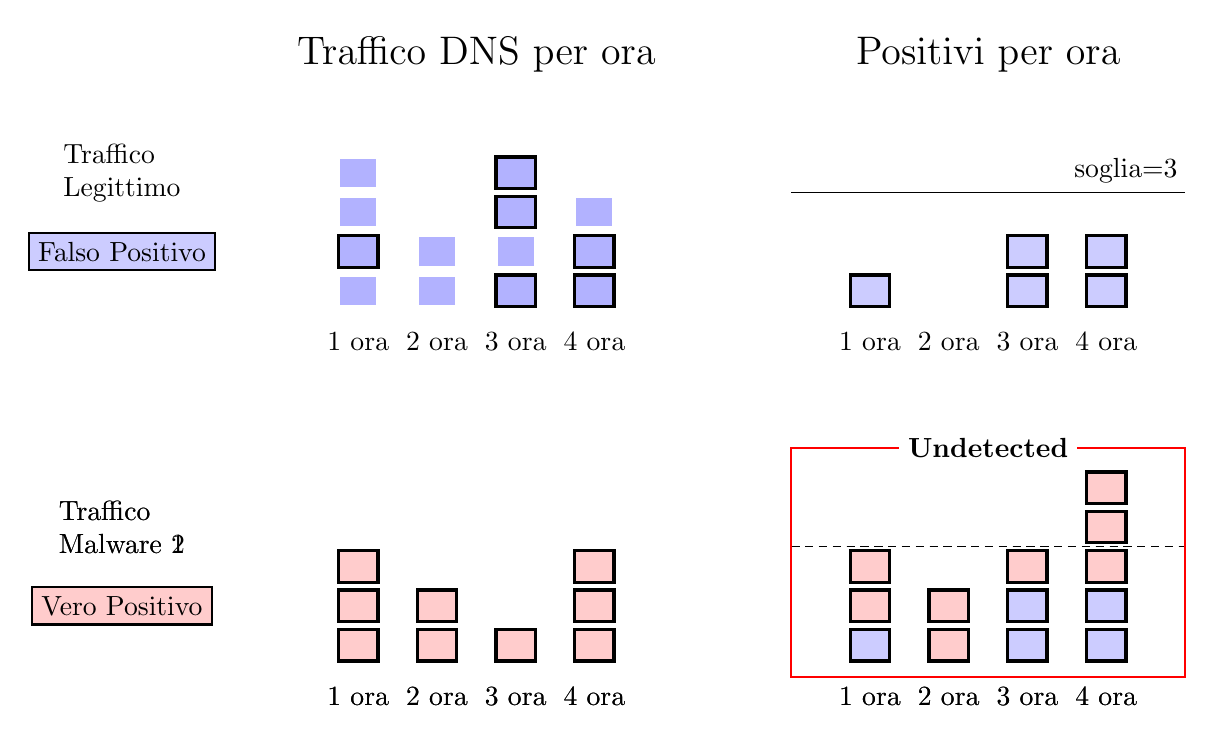
\begin{tikzpicture}

    \tikzset{
      pnode/.style={draw,minimum width=5mm,minimum height=4mm}
    }
    % \pic {ggrid};

    \def\neg{{0,1,0,0},{0,0},{1,0,1,1},{1,1,0}};
    \def\pos{{1,0,1},{1},{},{1,1,1}}
    \def\pn{1/2,0/1,3/0,2/3}

    \node[font=\Large] at ( 2, 3.5) {Traffico DNS per ora};
    \node[font=\Large] at (8.5, 3.5) {Positivi per ora};
    % \node[draw=white,thick,fill=blue!20] at ( 4, 3.5) {Vero Negativo};
    \node[draw,thick,fill=blue!20] at ( -2.5, 1) {Falso Positivo};
    % \node[draw=white,thick,fill=red!20] at ( 8, 3.5) {Falso Negativo};
    \onslide<3->{
      \node[draw,thick,fill=red!20] at ( -2.5, -3.5) {Vero Positivo};
    }

    \begin{scope}[xshift=0cm]
      \node[align=left] at (-2.5,2) {Traffico\\Legittimo};
      \foreach[count=\i] \arr in \neg {
        \foreach[count=\j] \x in \arr {
          \pgfmathsetmacro{\c}{\x == 0 ? "white" : "black"}
          \node[fill=blue!30,draw=\c,very thick,pnode] (n\i\j) at (\i-0.5,\j*5mm) {};
        }
        \node at (\i-0.5, -0.15) {\i\ ora};
      }

      \onslide<2->{
        \begin{scope}[xshift=6cm]
        \foreach[count=\i] \fp in {1,0,2,2} {
          \ifthenelse{\fp>0}{
            \foreach \j in {1,...,\fp} {
              \node[fill=blue!20,draw=black,very thick,pnode] (pp\i\j) at (\i,\j*5mm) {};
            }
          }{}
          \node at (\i, -0.15) {\i\ ora};
        }
        \draw [] (0,17.5mm) -- (5,17.5mm) node[above,pos=0.85] {soglia=3};
      \end{scope}
      }
    \end{scope}


    \begin{scope}[yshift=-4.5cm]
      \onslide<3-4>{
        \node[align=left] at (-2.5,2) {Traffico\\Malware 1};
        \foreach[count=\i] \arr in \pos {
          \foreach[count=\j] \x in \arr {
            \pgfmathsetmacro{\c}{\x == 0 ? "white" : "black"}
            \node[fill=red!20,draw=\c,very thick,pnode] (p\i\j) at (\i-0.5,\j*5mm) {};
          }
          \node at (\i-0.5, -0.15) {\i\ ora};
        }
      }

      \onslide<4>{
        \begin{scope}[xshift=6cm]
          \foreach[count=\i] \fp/\tp in \pn {
            \ifthenelse{\fp>0}{
              \foreach \j in {1,...,\fp} {
                \node[fill=blue!20,draw=black,very thick,pnode] (pp\i\j) at (\i,\j*5mm) {};
              }
            }{}
            \ifthenelse{\tp > 0}{
              \foreach \j in {1,...,\tp} {
                \pgfmathtruncatemacro{\jj}{\fp+\j}
                \node[fill=red!20,draw=black,very thick,pnode] (pp\i\jj) at (\i,\jj*5mm) {};
              }
            }{}
            \node at (\i, -0.15) {\i\ ora};
          }
          % \draw [dashed] (0,22.5mm) -- (5,22.5mm);
          \draw [densely dashed] (0,17.5mm) -- (5,17.5mm);
          \draw[ForestGreen,thick] (0, 0.1) rectangle (5, 3);
          \node[fill=white] at (2.5, 3) {\textbf{Detected}};
        \end{scope}
      }
    \end{scope}

    \def\neg{{0,1,0,0},{0,0},{0,1,0,1},{1,1,0,0}};
    \def\pos{{1,1},{1,1},{1},{1}}
    \def\pn{1/2,0/2,2/1,2/1}

    \begin{scope}[yshift=-4.5cm]
      \onslide<5-6>{
        \node[align=left] at (-2.5,2) {Traffico\\Malware 2};
        \foreach[count=\i] \arr in \pos {
          \foreach[count=\j] \x in \arr {
            \pgfmathsetmacro{\c}{\x == 0 ? "white" : "black"}
            \node[fill=red!20,draw=\c,very thick,pnode] (p\i\j) at (\i-0.5,\j*5mm) {};
          }
          \node at (\i-0.5, -0.15) {\i\ ora};
        }
      }

      \onslide<6>{
        \begin{scope}[xshift=6cm]
          \foreach[count=\i] \fp/\tp in \pn {
            \ifthenelse{\fp>0}{
              \foreach \j in {1,...,\fp} {
                \node[fill=blue!20,draw=black,very thick,pnode] (pp\i\j) at (\i,\j*5mm) {};
              }
            }{}
            \ifthenelse{\tp > 0}{
              \foreach \j in {1,...,\tp} {
                \pgfmathtruncatemacro{\jj}{\fp+\j}
                \node[fill=red!20,draw=black,very thick,pnode] (pp\i\jj) at (\i,\jj*5mm) {};
              }
            }{}
            \node at (\i, -0.15) {\i\ ora};
          }
          \draw [densely dashed] (0,17.5mm) -- (5,17.5mm);
          \draw[red,thick] (0, 0.1) rectangle (5, 3);
          \node[fill=white] at (2.5, 3) {\textbf{Undetected}};
        \end{scope}
      }
    \end{scope}
  \end{tikzpicture}%
  }
\end{center}
\end{frame}


\begin{frame}{Data set}


  \begin{center}
    \resizebox{\textwidth}{!}{%


    \begin{tikzpicture}

      \node at (-2,4) {%
      \parbox{9cm}{\begin{itemize}
        \item \ac{PCAP} da Stratosphere repository.
        \item Un tipo di traffico legittimo.
        \item Quattro diversi traffici malevoli.
        \begin{itemize}
          \item Malware \textit{caphaw}.
          \item Malware \textit{simda}.
          \item Malware \textit{virut}.
          \item Malware \textit{zbot}.
        \end{itemize}
      \end{itemize}}
      };

      \node[draw, rounded corners, text width=1.75cm] (lstm) at (4,4) {
\includegraphics[width=\textwidth]{ml.pdf}};
      \node[fill=white,font=\large] at (lstm.north) {\textbf{LSTM}};

      \node[text width=12cm] at (0,0) {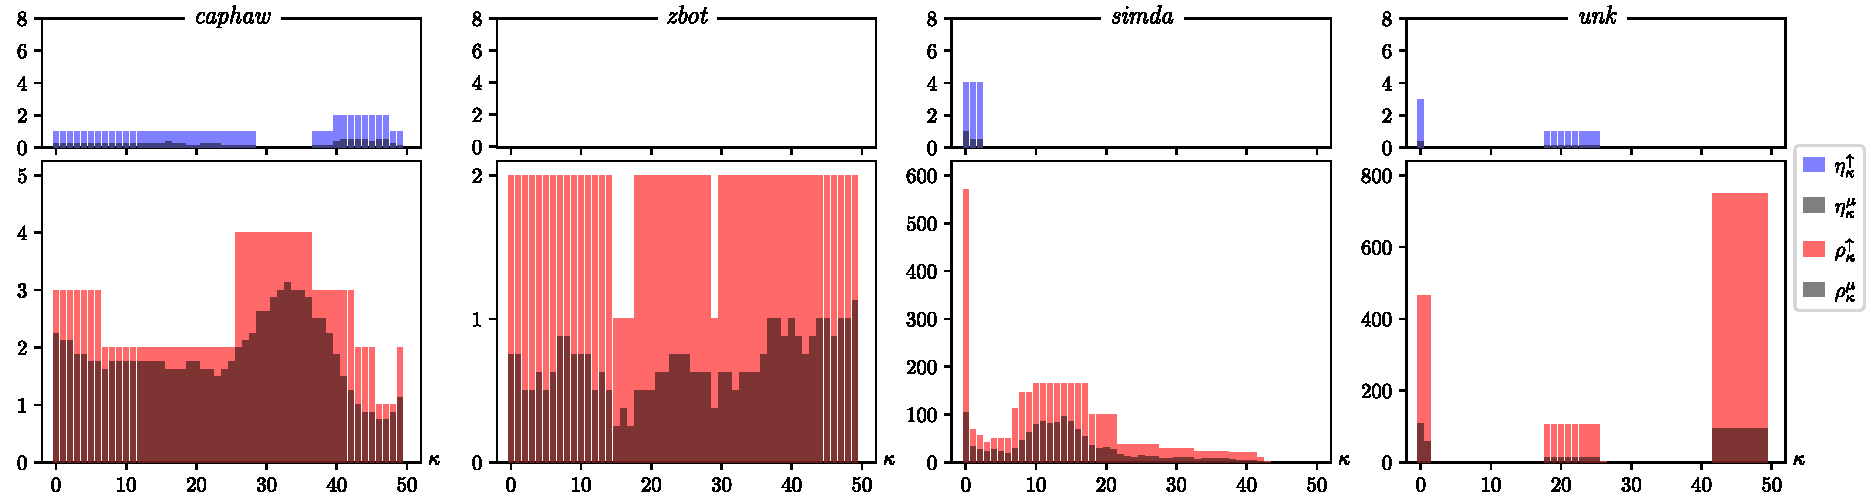
\includegraphics[width=1\textwidth]{malicious_s3.pdf}};
  \end{tikzpicture}
  }
\end{center}
\end{frame}


\begin{frame}{Conclusioni}
  \begin{center}
    \begin{tabular}{lllll}
      \textit{malware} & \phantom{ab} & TPR &\phantom{b} & \multicolumn{1}{p{3cm}}{Ore con attività malevola rilevate} \\\midrule
      caphaw      && 0.96 && 100\%    \\
      simda       && 0.95 && 86\%    \\
      virut       && 0.93 && 36\%    \\
      zbot        && 0.94 && 90\%    \\\bottomrule
    \end{tabular}
  \end{center}
  \begin{itemize}
    \item L'efficienza di rilevazione dipende dall'evoluzione temporale del traffico malevolo e benevolo.
    \item Necessario studio di una soglia dinamica.
    \item Necessario studio evoluzione temporale traffico benevolo e malevolo.
  \end{itemize}
\end{frame}



\section{Graph-based NIDS}

\begin{frame}{Tema 3}

  Sistema di rilevazione basato su monitoraggio traffico di rete utilizzando la Teoria dei Grafi.
    \begin{itemize}
      \item Si utilizza un grafo per modellare le connessioni che avvengono in una rete locale.
      \item \textbf{Obiettivo}: Sviluppare un classificatore binario (benevole/malevole) di connessioni basato solo su graph features.
      \item \textbf{Vantaggio}: non analizzando il contenuto dei pacchetti, supera le limitazioni di quando si utilizzano comunicazioni criptate o tecniche elusive.
    \end{itemize}
  
  \end{frame}
  
  \begin{frame}{Graph-based NIDS}
  
  \resizebox{\textwidth}{!}{%
  \begin{tikzpicture}
  
      % \pic {ggrid};
  
      \node[font=\Large] at (4,8) {Local Network};
      
      \pic (seagull) at (4, 4.5) {seagull};
      
      \pause
      
      \node[font=\Large] at (12,8) {Graph};
  
      \coordinate (g-origin) at (12, 4.5);
      \begin{scope}[xshift=12cm,yshift=4.5cm]
        \foreach[count=\i] \angle in {1,2,3,4,5,6} {
          \node[circle,draw=blue,thick,minimum width=0.5cm,inner sep=0] (gt\i) at (60*\angle:2cm) {\i};
        }
  
        \foreach[count=\i] \angle in {1,2,3,4,5,6} {
          \foreach[count=\j] \angle in {1,2,3,4,5,6} {
            \draw[<->,black!60] (gt\i) .. controls (0, 0) .. (gt\j);
          }
        }
      \end{scope}
  
      \pause
  
      \pgfmathsetmacro{\na}{2}
      \pgfmathsetmacro{\nb}{4}
  
      \onslide<3-4>{
        \draw[Stealth-Stealth,ultra thick, black!80] (seagull-t\na) .. controls (seagull-origin) .. (seagull-t\nb);
        \node[draw,font=\large] at(8,1.5) {connessione tra terminale \na\ e \nb};
      }
  
      \onslide<4>{
        \node[circle,fill=white,draw=blue,ultra thick, font=\bfseries, minimum width=0.5cm,inner sep=0] at (gt\na) {\na};
        \node[circle,fill=white,draw=blue,ultra thick, font=\bfseries, minimum width=0.5cm,inner sep=0] at (gt\nb) {\nb};
        \draw[Stealth-Stealth,ultra thick, black!80] (gt\na) .. controls (g-origin) .. (gt\nb);
        \draw[->,ultra thick] (7,4.5) -- (9,4.5) node[midway,above,font=\large]{update};
      }
  
      \pgfmathsetmacro{\na}{1}
      \pgfmathsetmacro{\nb}{6}
      \onslide<5-6>{
        \draw[Stealth-Stealth,ultra thick, black!80] (seagull-t\na) .. controls (seagull-origin) .. (seagull-t\nb);
        \node[draw,font=\large] at(8,1.5) {connessione tra terminale \na\ e \nb};
      }
  
      \onslide<6>{
        \pgfmathsetmacro{\na}{1}
        \pgfmathsetmacro{\nb}{6}
        \node[circle,fill=white,draw=blue,ultra thick, font=\bfseries, minimum width=0.5cm,inner sep=0] at (gt\na) {\na};
        \node[circle,fill=white,draw=blue,ultra thick, font=\bfseries, minimum width=0.5cm,inner sep=0] at (gt\nb) {\nb};
        \draw[Stealth-Stealth,ultra thick, black!80] (gt\na) .. controls (g-origin) .. (gt\nb);
        \node[draw,font=\large] at(8,1.5) {connessione tra terminale \na\ e \nb};
        \draw[->,ultra thick] (7,4.5) -- (9,4.5) node[midway,above,font=\large]{update};
      }
  \end{tikzpicture}%
  }
  \end{frame}
  
  
  \begin{frame}{Graph-based NIDS}
    \resizebox{\textwidth}{!}{%
    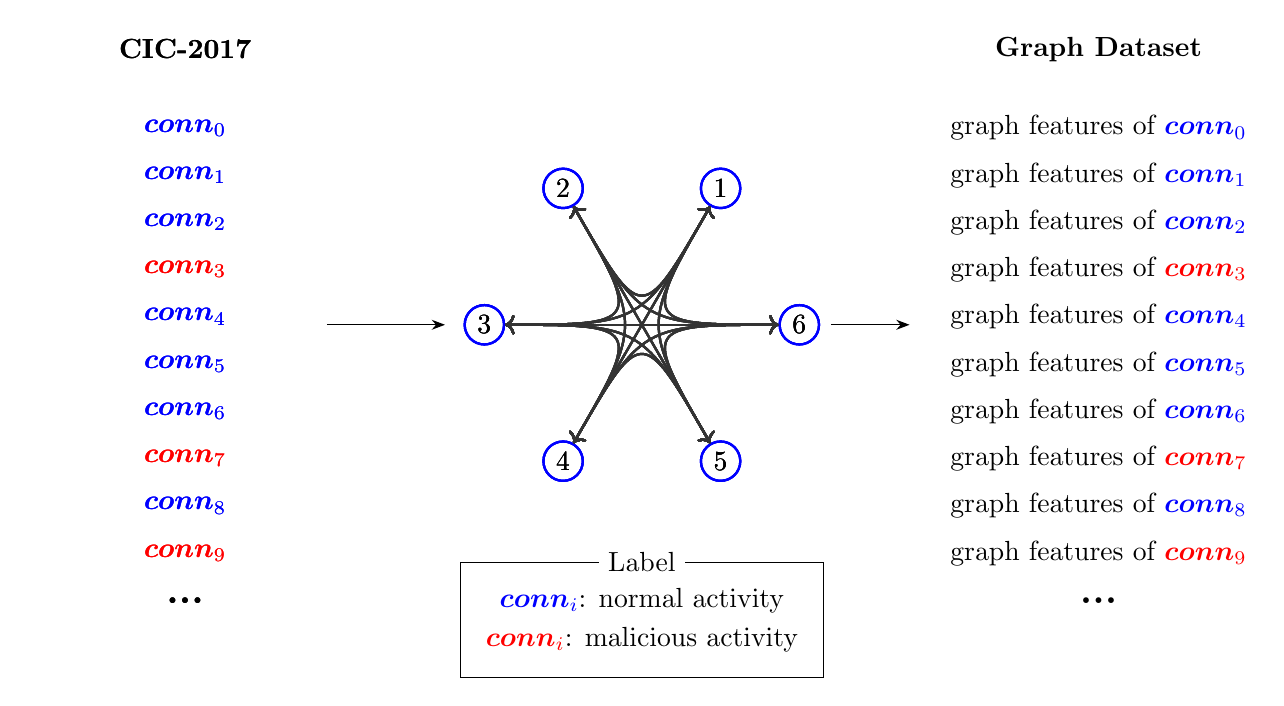
\begin{tikzpicture}
      % \pic at (0,0) {ggrid};
  
      \node[] (ln) at (8,1) {\textcolor{blue}{$\bm{conn}_i$}: normal activity};
      \node[] (lm) at (8,0.5) {\textcolor{red}{$\bm{conn}_i$}: malicious activity};
      \node[draw,inner sep=.2cm, fit=(ln) (lm)] (lfit) {};
      \node[fill=white] at(lfit.north) {Label};
  
      \onslide<1>{
        \pic at (2.2,0) {cdataset};
        \pic at (8,4.5) {ggraphempty};
        % \draw[-Stealth] (4,4.5) -- (5.5,4.5);
      }
  
      \onslide<2>{
        \pic at (2.2,0) {cdataset};
        \pic at (8,4.5) {ggraph};
        \draw[-Stealth] (4,4.5) -- (5.5,4.5);
      }
  
      \onslide<3>{
        \pic[opacity=0.2] at (2.2,0) {cdataset};
        \pic at (13.8,0) {gdataset};
        \pic at (8,4.5) {ggraph};
        \draw[-Stealth] (10.4,4.5) -- (11.4,4.5);
      }
  
    \end{tikzpicture}%
    }
  \end{frame}
  
  
  \begin{frame}{Graph-based NIDS}
    \resizebox{\textwidth}{!}{%
    \begin{tikzpicture}
      % \pic at (0,0) {ggrid};
  
      \onslide<1>{
        
        \node[font=\large,align=center] (split) at (8,8.5) {Graph dataset split};
        \pic (gdataset) at (2.2,0) {gdataset}; \node (train) at (2,8.4) {\textbf{Training}};
        \pic (gdatasettest) at (14,0) {gdatasettest}; \node (test) at (14,8.4) {\textbf{Test}};
        \draw[->, thick] (split.west) -- ++(-2.5cm,-0.2cm);
        \draw[->, thick] (split.east) -- ++(2.5cm,-0.2cm);
  
      }
  
      \onslide<2>{
        \pic (gdataset) at (2.2,0) {gdataset}; \node (train) at (2,8.4) {\textbf{Training}};
        \pic[opacity=0.3] (gdatasettest) at (14,0) {gdatasettest}; \node[opacity=0.3] (test) at (14,8.4) {\textbf{Test}};
  
        \node[draw, rounded corners, text width=1.5cm, inner sep=0.2cm, font=\Huge] (svm) at (8,4.5) {
\includegraphics[width=\textwidth]{ml.pdf}}; \node[fill=white,font=\large] at (svm.north) {\textbf{SVM}};
  
        \draw[-Stealth, ultra thick] (4.2,4.5) -- (7,4.5) node[above,midway,font=\large] {training};
      }
      
  
      \onslide<3>{
        \pic[opacity=0.3] (gdataset) at (2.2,0) {gdataset}; \node[opacity=0.3] (train) at (2,8.4) {\textbf{Training}};
        \pic (gdatasettest) at (14,0) {gdatasettest}; \node (test) at (14,8.4) {\textbf{Test}};
  
        \node[draw, rounded corners, text width=1.5cm, inner sep=0.2cm, font=\Huge] (svm) at (8,4.5) {
\includegraphics[width=\textwidth]{ml.pdf}}; \node[fill=white,font=\large] at (svm.north) {\textbf{SVM}};
  
        \draw[Stealth-, ultra thick] (9,4.5) -- (12,4.5) node[above,midway,font=\large] {testing};
      }
  
  
      
  
    \end{tikzpicture}%
    }
  \end{frame}
  
  \begin{frame}{Graph-based NIDS: risultati}
    \begin{center}
      \begin{tabular}{llr}
      \multicolumn{3}{l}{\textbf{SVM test metrics}} \\\midrule
      \multicolumn{2}{l}{F1 weighted avg} & \textbf{0.9988} \\[2mm]
      \multicolumn{3}{l}{Negatives/Benign} \\
       & False Positives & 272 \\
       & F1 score & 0.9991 \\
       & False Positive Ratio & 0.0002 \\[2mm]
      \multicolumn{3}{l}{Positives/Attacks} \\
       & False negatives & 2016 \\
       & F1 & 0.9979 \\
       & False Negative Ratio & 0.0037 \\ \bottomrule
      \end{tabular}
    \end{center}
  \end{frame}
  
  

% \begin{frame}
% Ricerca Venezia
% \begin{itemize}
%        \item traffico reale.
%        \item uso LLR.
%        \item detection senza falsi positivi possibile.
% \end{itemize}
% \end{frame}


% \begin{frame}
%        Ricerca Malesia
%        \begin{itemize}
%               \item traffico reale su traffico malevolo.
%               \item traffico reale può compromettere la rilevazione.
%        \end{itemize}
% \end{frame}



\section{Collaborazioni}
\begin{frame}{Attività di ricerca: collaborazione con aziende}
  Collaborazione con aziende o enti pubblici:
  \begin{itemize}
      \item ASTEA SPA:
      \begin{itemize}
          \item implementazione di applicazioni SIEM QRadar, Netbox.
          \item sviluppo applicazione per controllo vulnerabilità degli assets dell'azienda.
      \end{itemize}
      \item Ancharia SRL: applicazione per la valutazione della sicurezza di un ente o un'azienda a partire dal suo dominio web, recuperando
      dati di vulnerabilità e data breach da fonti di Open-Source Intelligence (OSINT).
      \item Regione Marche: studio per l'implementazione di uno CSIRT regionale.
      \item Montimage SRL, Parigi: sviluppo di un test-bed per esperimenti di NIDS su Blockchain DNS.
  \end{itemize}
\end{frame}

\section{Pubblicazioni}
  \begin{frame}{Attività di ricerca: collaborazione con aziende}
    Atti di congresso internazionale censito nei database ISI:
    \begin{itemize}
      \item L. Principi, M. Baldi, A. Cucchiarelli, L. Spalazzi, “Efficiency of Malware Detection based on DNS Packet Analysis over Real Network Traffic”, Proc. IEEE CSR 2023, Venice, Italy, July 31 - August 2, 2023.
      \item Zonneveld G., Principi L., Baldi L., “Using Graph Theory for Improving Machine Learning based Detection of Cyber Attacks”, Proc. IEEE ICMLCN 2024, Stockholm, Sweden, May 2024.
      \item L. Principi, M. Baldi, “Applying Intrusion Detection based on Algorithmically Generated Domain Classification to Real Network Traffic”, Proc. IEEE CyberComp 2024, Melaka, Malaysia, 6 - 7 November, 2024.
    \end{itemize}
  \end{frame}

\end{document}